\documentclass[12pt]{article}
\usepackage[left=2cm, right=2cm]{geometry}
\usepackage[portuguese]{babel}
\usepackage{amsmath}
\usepackage{amsfonts}
\usepackage{booktabs}
\usepackage{adjustbox}
\usepackage{graphicx}
\usepackage{array}
\usepackage{float}

% Define a new column type with right alignment
\newcolumntype{R}[1]{>{\raggedleft\arraybackslash}p{#1}}

\title{Relatório Trabalho Final – Problema 1: Fábrica de papel}
\author{
    Henrique Santa Terra \\
    Jenice Júlio Correa de Lima \\
    José Nivaldo da Silva Hypólito \\
    Luciene Alves Santos Mota \\
    Paula Lumy Takeuchi \\
    Prof.  Me.  Júnior César Bonafim (jrbonafim@gmail.com) 
}


\begin{document}
\maketitle

\newpage
\section{Apresentação do problema} %%%%%%%%%%%%%%%%%%%%%%%%%%%%%%%%%%%%%%%%%%%%%%%%%%%%%%%%%%%%%%%%%%%%%
O problema recebido se trata sobre uma fábrica que necessita cortar matrizes de 
papel de acordo com a demanda de itens menores. O problema é dividido em duas partes, 
a parte A requer a minimização do desperdício de papel da matriz que será cortada 
de acordo com os padrões de corte, a parte B possui o mesmo segmento da parte A 
com a introdução de uma nova variável que limita a quantidade de padrões de corte.\\

Os arquivos com os dados utilizados para a resolução do problema foram disponibilizados da seguinte forma:\\

\begin{figure}[h]
    \centering
    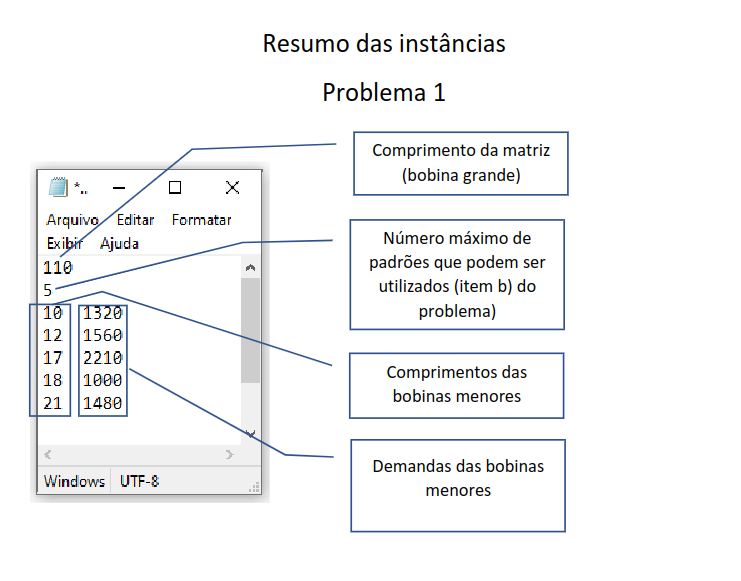
\includegraphics[width=0.5\textwidth]{input.png}
    \caption{Resumo das instâncias}
\end{figure}

Também foi passado uma dica para a resolução do problema envolvendo o uso de combinações 
para gerar os possíveis padrões de corte.\\

\newpage

\section{Resolução do problema A} %%%%%%%%%%%%%%%%%%%%%%%%%%%%%%%%%%%%%%%%%%%%%%%%%%%%%%%%%%%%%%%%%%%%%
Com base nos parâmetros definidos na apresentação do problema o seguinte modelo foi criado:

\textbf{Quantidades}
\begin{itemize}
    \item $n$: Quantidade de tipos de itens
    \item $m$: Quantidade de padrões de corte
\end{itemize}

\textbf{Variáveis}
\begin{itemize}
    \item $x_j$: Quantidade que será utilizada do padrão de corte $j$, para $j = 1,\ldots, m$
\end{itemize}

\textbf{Parâmetros}
\begin{itemize}
    \item $D_i$: Demanda do item $i$, para $i = 1,\ldots, n$
    \item $P_{ij}$: Padrão de corte $i$ do tipo de item $j$, para $i = 1,\ldots, n$ e $j = 1,\ldots, m$
\end{itemize}

\textbf{Modelo}
\begin{align*}
    \hbox{min} \ \ 
        & \sum_{j=1}^m x_i \\
    \hbox{s.a.} \ \ 
        & \sum_{j=1}^m P_{ij} x_j \geq D_i && i = 1,\ldots, n \\
        & x_{j} \in +\mathbb{Z}            && j = 1,\ldots, m \\
\end{align*}

Após a realização dos testes os seguintes resultados foram obtidos:
\begin{table}[H]
    \centering
    \caption{Resultados obtidos após a realização dos testes para a parte A do problema}
    \adjustbox{max width=\textwidth}{
        \begin{tabular}{| l | p{3cm} p{3cm} p{3cm} p{4cm} p{3cm} p{3cm} |}
            \toprule
            Arquivos & Tamanho da matriz & Qnt. de itens menores & Qtn. de padrões de corte gerados & Qtn. de padrões de corte utilizados & Total de matrizes usadas & Qtn. de papel desperdiçada \\
            \midrule
            inst\_200\_5.txt & 200 & 5 & 51 & 8 & 3339 & 18957 \\
            inst\_130\_6.txt & 130 & 6 & 48 & 6 & 5135 & 5946 \\
            inst\_200\_4.txt & 200 & 4 & 14 & 3 & 3381 & 13826 \\
            inst\_110\_5.txt & 110 & 5 & 229 & 9 & 1078 & 0 \\
            inst\_100\_4.txt & 100 & 4 & 24 & 4 & 2194 & 10943 \\
            inst\_250\_5.txt & 250 & 5 & 64 & 6 & 3078 & 11698 \\
            inst\_100\_6.txt & 100 & 6 & 91 & 7 & 3128 & 6106 \\
            inst\_130\_4.txt & 130 & 4 & 14 & 4 & 3081 & 6938 \\
            inst\_250\_6.txt & 250 & 6 & 119 & 9 & 3090 & 3004 \\
            inst\_200\_6.txt & 200 & 6 & 87 & 6 & 4084 & 15757 \\
            inst\_130\_5.txt & 130 & 5 & 38 & 5 & 3468 & 2613 \\
            inst\_100\_5.txt & 100 & 5 & 40 & 6 & 2678 & 12879 \\
            inst\_250\_4.txt & 250 & 4 & 25 & 5 & 2448 & 22514 \\
            \bottomrule
        \end{tabular}
    }
\end{table}

A partir os resultados obtidos para a parte A do problema, observa-se que a instância inst\_110\_5.txt, 
com  matriz de tamanho 110 e com 5 tamanhos diferentes de itens menores, se destaca das demais por sua 
grande quantidade de padrões de cortes gerados, 229, o que levou a minimizar o uso de matrizes, com 1078 
bobinas grandes usadas, e ao não desperdício de papel. Essa instância também apresentou uma rápida 
resolução do problema com um número pequeno de iterações.

\newpage

\section{Resolução do problema B} %%%%%%%%%%%%%%%%%%%%%%%%%%%%%%%%%%%%%%%%%%%%%%%%%%%%%%%%%%%%%%%%%%%%%
Com base nos parâmetros definidos na apresentação do problema o seguinte modelo foi criado:

\textbf{Quantidades}
\begin{itemize}
    \item $n$: Quantidade de tipos de itens
    \item $m$: Quantidade de padrões de corte
\end{itemize}

\textbf{Variáveis}
\begin{itemize}
    \item $x_j$: Quantidade que será utilizada do padrão de corte $j$, para $j = 1,\ldots, m$  
    \item $s_j = 
        \begin{cases}
            1 : \text{Caso o padrão } j \text{ seja utilizado} \\
            0 : \text{Caso não seja}
        \end{cases}
    $
\end{itemize}

\textbf{Parâmetros}
\begin{itemize}
    \item $D_i$: Demanda do item $i$, para $i = 1,\ldots, n$  
    \item $P_{ij}$: Padrão de corte $i$ do tipo de item $j$, para $i = 1,\ldots,n$ e $j = 1,\ldots,m$  
    \item $R$: Máximo permitido de padrões de corte  
\end{itemize}

\textbf{Modelo}
\begin{align*}
    \hbox{min} \ \ 
        & \sum_{j=1}^m x_i \\
    \hbox{s.a.} \ \ 
        & \sum_{j=1}^m P_{ij} x_j \geq D_i && i = 1, \ldots, n \\
        & \sum_{j=1}^m s_j \leq R                              \\
        & x_j \leq M s_j                   && j = 1, \ldots, m \\
        & M = \sum_{i=1}^n D_i                                 \\
        & s_j \in \{0, 1\}                 && j = 1, \ldots, m \\
        & x_{j} \in +\mathbb{Z}            && j = 1, \ldots, m \\
\end{align*}

Após a realização dos testes os seguintes resultados foram obtidos:
\begin{table}[htbp]
    \centering
    \caption{Resultados obtidos após a realização dos testes para a parte B do problema}
    \adjustbox{max width=\textwidth}{
        \begin{tabular}{| l | p{2cm} p{4cm} p{3cm} p{3.5cm} p{3.5cm} p{2.5cm} p{3cm} |}
            \toprule
            Arquivos & Tamanho da matriz & Qtn. de itens menores & Qtn. de padrões de corte gerados & Limite de Padrões de corte & Qtn. de padrões de corte utilizados & Total de matrizes usadas & Qtn. de papel desperdiçada \\
            \midrule
            inst\_200\_5.txt & 200 & 5 & 51 & 5 & 5 & 4201 & 15524 \\
            inst\_130\_6.txt & 130 & 6 & 48 & 7 & 7 & 5135 & 5956 \\
            inst\_200\_4.txt & 200 & 4 & 14 & 4 & 3 & 3381 & 13826 \\
            inst\_110\_5.txt & 110 & 5 & 229 & 5 & 5 & 1079 & 0 \\
            inst\_100\_4.txt & 100 & 4 & 24 & 5 & 4 & 2194 & 10943 \\
            inst\_250\_5.txt & 250 & 5 & 64 & 5 & 5 & 3084 & 11108 \\
            inst\_100\_6.txt & 100 & 6 & 91 & 6 & 6 & 3129 & 6110 \\
            inst\_130\_4.txt & 130 & 4 & 14 & 5 & 5 & 3081 & 6947 \\
            inst\_250\_6.txt & 250 & 6 & 119 & 7 & 7 & 3090 & 3041 \\
            inst\_200\_6.txt & 200 & 6 & 87 & 6 & 6 & 4275 & 12224 \\
            inst\_130\_5.txt & 130 & 5 & 38 & 5 & 5 & 3468 & 2613 \\
            inst\_100\_5.txt & 100 & 5 & 40 & 6 & 6 & 2678 & 12879 \\
            inst\_250\_4.txt & 250 & 4 & 25 & 4 & 4 & 2449 & 22513 \\
            \bottomrule
        \end{tabular}
    }
\end{table}

Limitando o padrão de corte a 5, novamente, a instância inst\_110\_5.txt se destacou porque conseguiu minimizar 
o número de bobinas utilizadas, mantendo o mesmo resultado do item anterior e, também por ter mantido baixo o 
desperdício. Com a restrição, houve um grande aumento do tempo para a resolução, demorando muito mais que o 
resultado anterior e utilizando mais de 200 mil iterações do método simplex.

\newpage

\section{Conclusão} %%%%%%%%%%%%%%%%%%%%%%%%%%%%%%%%%%%%%%%%%%%%%%%%%%%%%%%%%%%%%%%%%%%%%

A partir dos resultados obtidos, pode-se concluir que apesar da restrição imposta na parte B do problema, 
foi possível manter a quantidade de bobinas utilizadas ao custo do aumento do desperdício de papel e aumento 
do tempo de processamento.

\end{document}
